% Section 5.1: paragraph, table, and figure environments in one copyable block.
% Required preamble packages: graphicx, subcaption, booktabs, threeparttable.
% Upload the five referenced figure PDFs under figures/conditions/ in Overleaf.
% Both the compact table and per-instance figure are retained as requested.
% BEGIN OVERLEAF CONTENT
\begingroup
\graphicspath{{figures/conditions/}{../figures/}}

% Draft for Section 5.1. Both decomposition presentations are retained for review.
% If choosing the table alone, replace "Figure~\ref{fig:penalty_parts} and
% Table~\ref{tab:penalty_summary}" with "Table~\ref{tab:penalty_summary}" below.
\paragraph{Operational interpretation.}
Under the base configuration, most charging is accommodated within driver
interruptions. Pooling charged energy across all 43 instances, 70.5\% is supplied
during daily rests and 24.9\% during breaks, leaving 4.7\% to be charged outside
either interruption (Figure~\ref{fig:charge_split}). These uncovered charging
sessions nevertheless account for 18.8\% of the 324 charging stops, indicating
that they tend to be relatively small top-ups. Figure~\ref{fig:penalty_parts} and
Table~\ref{tab:penalty_summary} decompose the resulting route time penalty into
uncovered charging time and additional break time. Within every electric--diesel
pair, total driving, customer service, and daily rest times are identical; the
two components therefore account for the entire penalty. Additional breaks
contribute 41.8\% of the pooled additional minutes. Fully synchronized charging
can thus still produce a longer route duration: charging may fit entirely
within a break that is additional to the diesel schedule. Of the 18 instances
in which all charging overlaps breaks or rests, seven still incur a positive
time penalty through additional breaks. The examples in
Figure~\ref{fig:operations} illustrate the distinction. Charging within daily
rests allows the electric schedule to match the diesel duration in
Figure~\ref{fig:rest_overlap}, whereas an uncovered top-up adds 15.33~minutes in
Figure~\ref{fig:early_charge}. In Figure~\ref{fig:extra_breaks}, all seven charging
sessions fit within breaks, but the electric schedule takes seven breaks
compared with three for diesel. The four additional 45-minute breaks explain
the full 180-minute penalty. Synchronization should therefore be assessed
jointly with the interruption pattern: a high share of overlapping charging
alone does not imply a small route time penalty.

% Charging split
\begin{figure}[tbp]
    \centering
    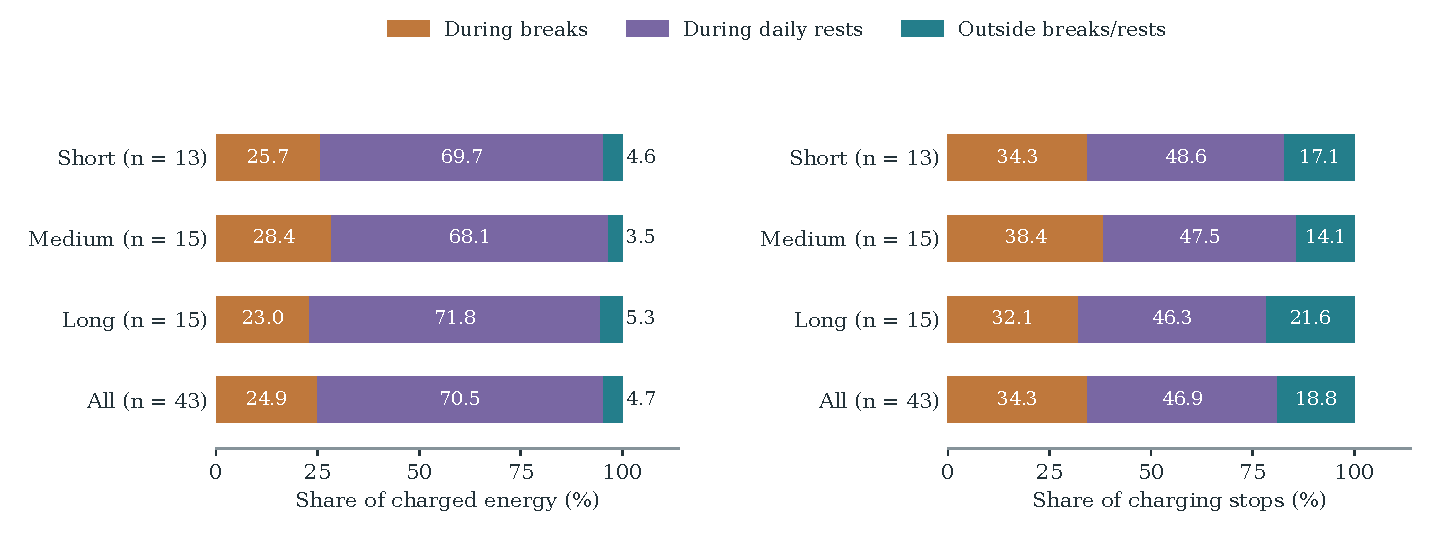
\includegraphics[width=\linewidth]{charge_split.pdf}
    \caption{Charging during breaks, during daily rests, and outside either, by route class and overall. The left panel pools charged energy; the right pools charging-stop counts. Sample sizes refer to instances. Constant charging power means energy shares also equal physical charging-time shares. Shares describe the saved minimum-time paths and are not averages of instance-level percentages. The base configuration is 750~kWh battery capacity, 350~kW charging power, 60~km maximum charging-station spacing, and 1.49~kWh/km energy consumption.}
    \label{fig:charge_split}
\end{figure}

% Compact decomposition table
\begin{table}[tbp]
    \centering
    \begin{threeparttable}
    \caption{Base-case sources of additional route time relative to diesel, by route class.}
    \label{tab:penalty_summary}
    \small
    \setlength{\tabcolsep}{4pt}
    \begin{tabular}{@{}lrrrrrr@{}}
    \toprule
    Route class & $n$ & \multicolumn{2}{c}{Instances with} & \multicolumn{3}{c}{Mean additional time (min)} \\
    \cmidrule(lr){3-4}\cmidrule(l){5-7}
     & & No penalty & Extra breaks & Charging & Breaks & Total \\
    \midrule
    Short & 13 & 8 & 0 & 7.4 & 0.0 & 7.4 \\
    Medium & 15 & 3 & 3 & 14.2 & 18.0 & 32.2 \\
    Long & 15 & 0 & 8 & 42.0 & 27.0 & 69.0 \\
    \midrule
    \textbf{All instances} & \textbf{43} & \textbf{11} & \textbf{11} & \textbf{21.8} & \textbf{15.7} & \textbf{37.5} \\
    \bottomrule
    \end{tabular}
    \begin{tablenotes}[flushleft]\footnotesize
    \item Charging denotes time spent charging outside breaks and daily rests; Breaks denotes additional break time relative to diesel. Their sum equals the total penalty. Driving, customer-service, and daily-rest durations are identical within each electric--diesel pair.
    \item Means include every instance in the indicated class, including zero penalties. The overall row weights all 43 instances equally. Extra breaks counts instances with at least one additional break, including those that also incur uncovered charging time.
    \end{tablenotes}
    \end{threeparttable}
\end{table}

% Alternative per-instance decomposition figure
\begin{figure}[tbp]
    \centering
    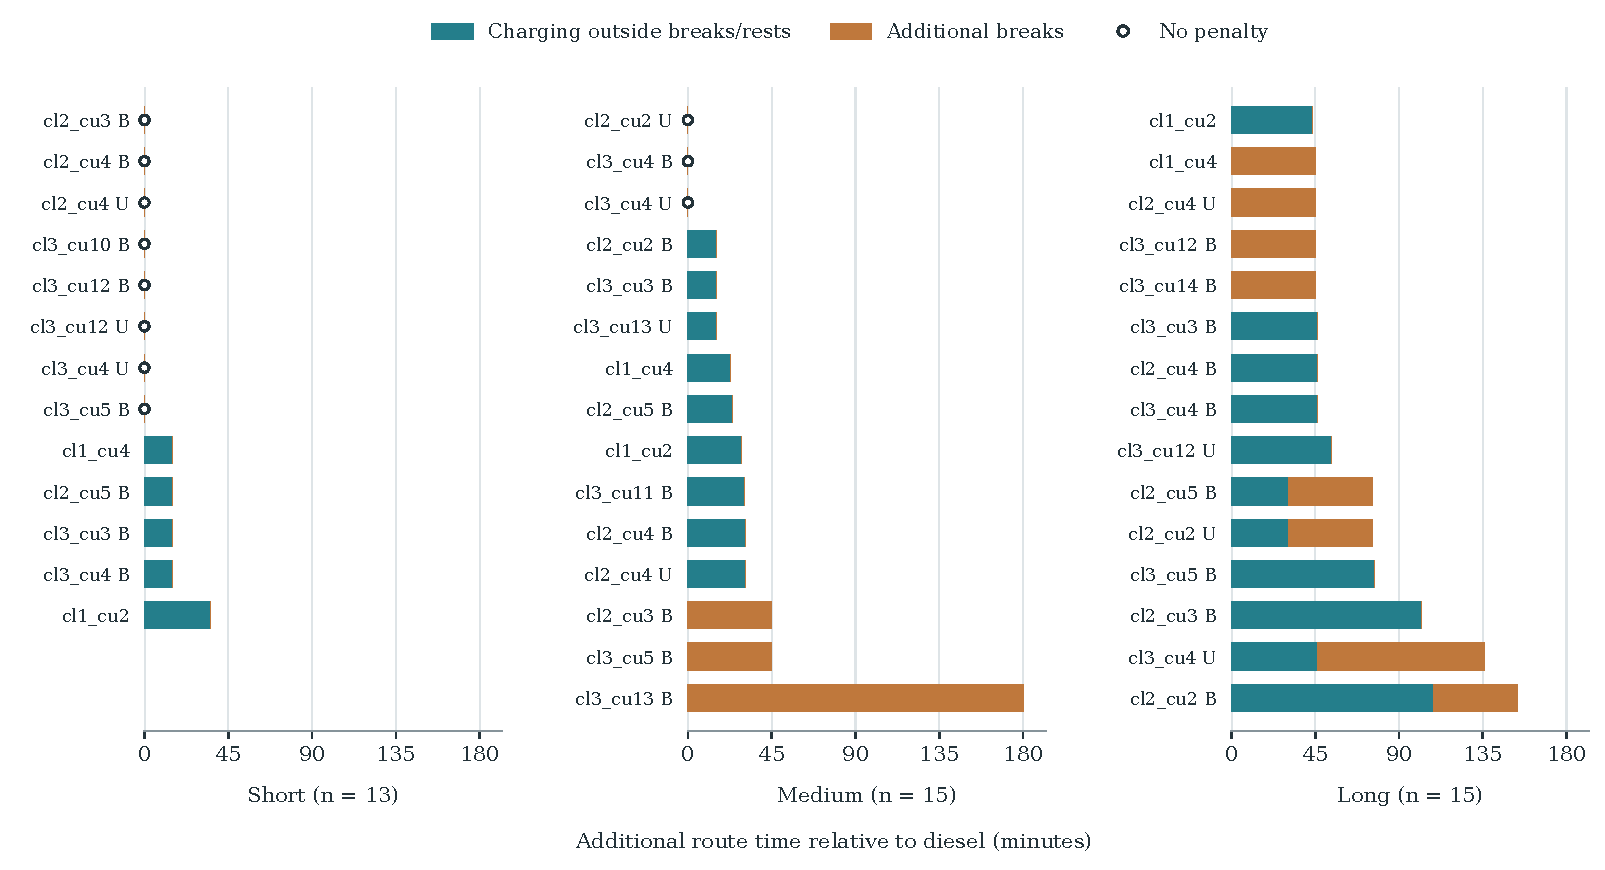
\includegraphics[width=\linewidth]{penalty_parts.pdf}
    \caption{Decomposition of additional route time relative to diesel for all 43 instances. Bars separate charging outside breaks/rests from additional break time. Open circles mark zero penalty. Driving, service, and daily-rest durations are unchanged within each pair. Instance labels omit the route class; B and U denote Balanced and Unbalanced. The base configuration is 750~kWh battery capacity, 350~kW charging power, 60~km maximum charging-station spacing, and 1.49~kWh/km energy consumption.}
    \label{fig:penalty_parts}
\end{figure}

% Three schedule examples
\begin{figure}[tbp]
    \centering
    \begin{subfigure}{\linewidth}
        \centering
        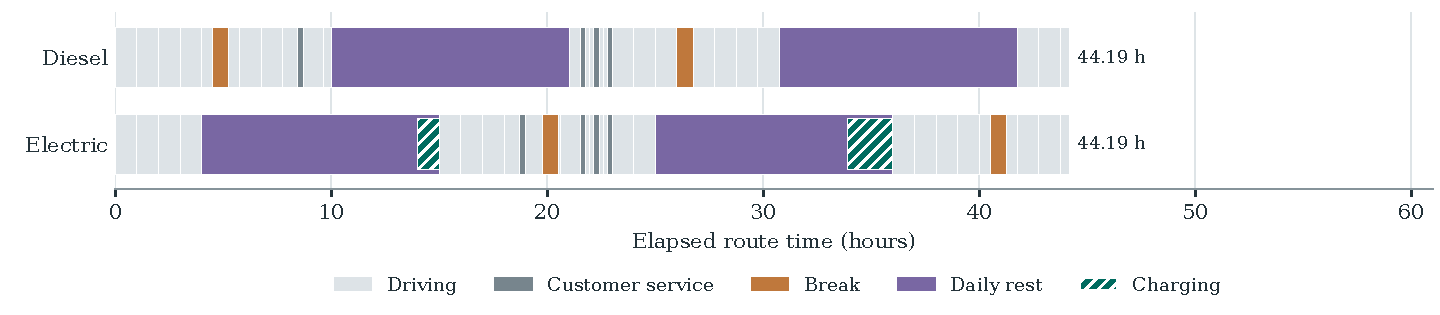
\includegraphics[width=\linewidth,trim=0 20bp 0 0,clip]{rest_overlap.pdf}
        \caption{Charging within daily rests (\texttt{short\_cl2\_cu4\_Balanced}).}
        \label{fig:rest_overlap}
    \end{subfigure}
    \medskip
    \begin{subfigure}{\linewidth}
        \centering
        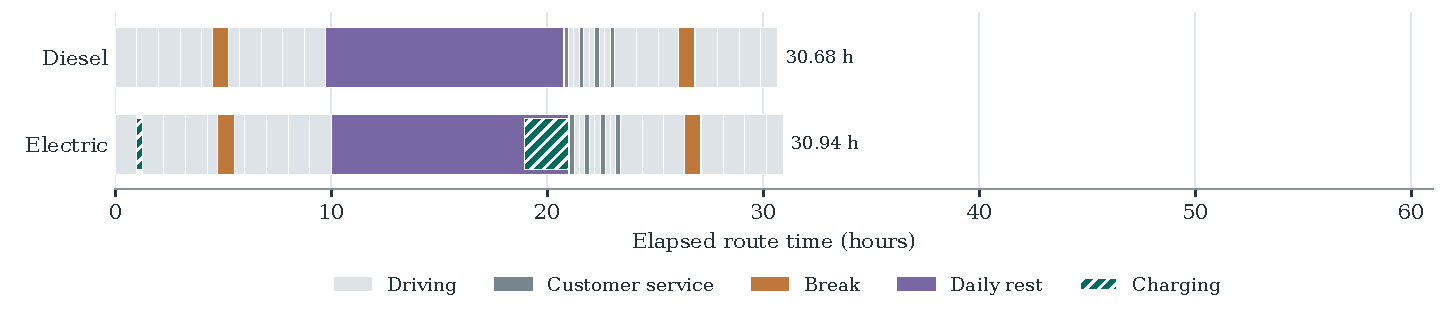
\includegraphics[width=\linewidth,trim=0 20bp 0 0,clip]{early_charge.pdf}
        \caption{Charging outside breaks and rests (\texttt{short\_cl1\_cu4}).}
        \label{fig:early_charge}
    \end{subfigure}
    \medskip
    \begin{subfigure}{\linewidth}
        \centering
        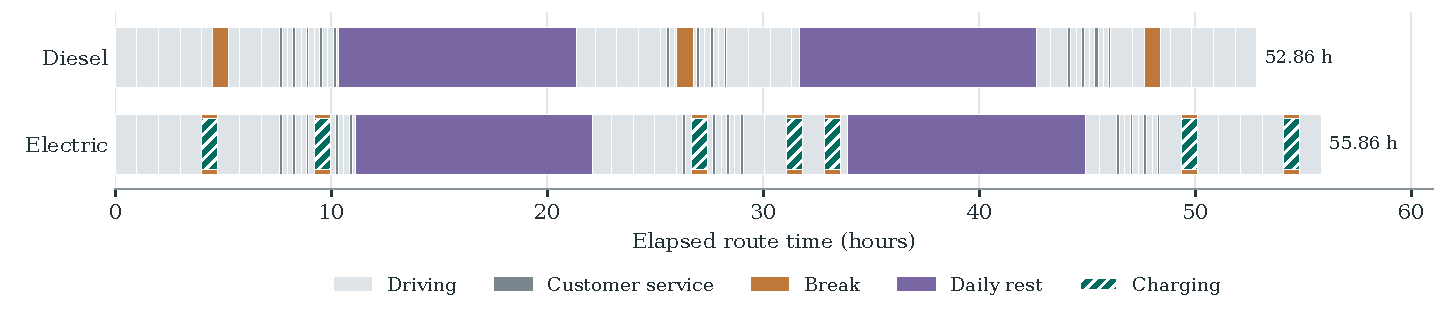
\includegraphics[width=\linewidth,trim=0 20bp 0 0,clip]{extra_breaks.pdf}
        \caption{Charging within additional breaks (\texttt{med\_cl3\_cu13\_Balanced}).}
        \label{fig:extra_breaks}
    \end{subfigure}
    \medskip
    % One shared legend: retain only the legend band from the final PDF.
    % All three schedule PDFs are 151.2bp tall; their bottom 20bp contain the legend.
    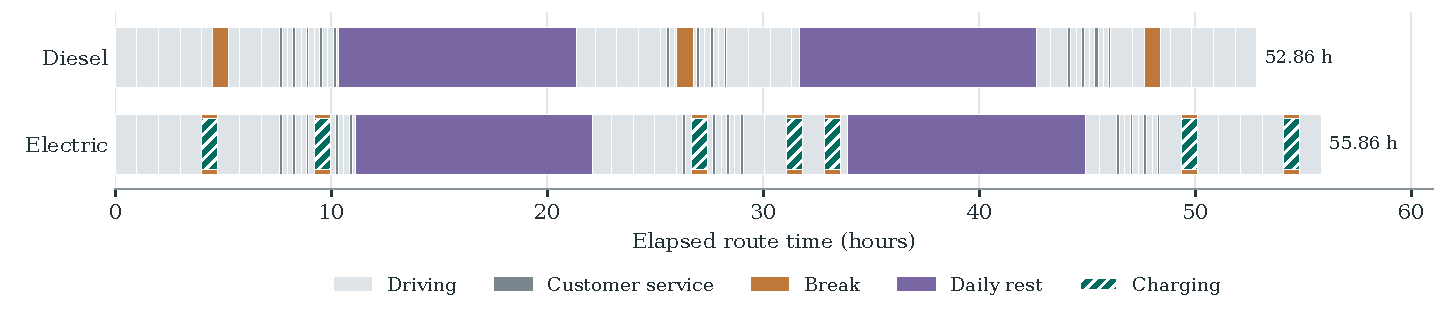
\includegraphics[width=\linewidth,trim=0 8bp 0 131.2bp,clip]{extra_breaks.pdf}\par
    \smallskip
    \caption{Three illustrative electric--diesel schedule pairs. The base configuration is 750~kWh battery capacity, 350~kW charging power, 60~km maximum charging-station spacing, and 1.49~kWh/km energy consumption. Dark teal regions with diagonal hatching show physical charging time reconstructed from charged energy and power. These regions cover most of the activity-bar height while retaining the actual charging duration on the time axis. Charging during daily rest is placed at the end of that rest for display; its exact position within the rest is not unique. All panels use the same time scale. The plots follow the recorded minimum-time paths; interval maxima are not combined with them. Examples illustrate observed mechanisms and are not representative frequency estimates.}
    \label{fig:operations}
\end{figure}

\endgroup
% END OVERLEAF CONTENT
